\documentclass[a4paper]{article}

\usepackage[english]{babel}
\selectlanguage{english}

\usepackage{pdfpages}
\usepackage{amssymb}
\usepackage[colorlinks]{hyperref}
\usepackage{cleveref}
\usepackage{cite}
\usepackage{verbatim}
\usepackage{fancyvrb}
\usepackage{tikz}
\usepackage[utf8x]{inputenc}
\usepackage{textcomp}
\usepackage{ucs}

\usetikzlibrary{backgrounds,calc}

\newcommand{\MPass}{\textsc{MPass}}
\newcommand{\binary}{MPass}
\newcommand{\transition}{t}
\newcommand{\occvar}{{\tt occ}}
\newcommand{\occvarof}[1]{\occvar\left({#1}\right)}
\newcommand{\indexvar}{{\tt index}}
\newcommand{\indexvarof}[1]{\indexvar\left({#1}\right)}
\newcommand{\matchingvar}{{\tt match}}
\newcommand{\matchingvarof}[1]{\matchingvar\left({#1}\right)}
\newcommand{\implies}{\Longrightarrow}

\title{MPass: \large{An efficient and computational tool for analysis of message passing programs}\\\small{User Manual}}
\author{Gaurav Saini and Subham Modi}

\begin{document}

\maketitle

\pagebreak

\begin{Verbatim}[fontsize=\small]
Copyright (C) 2013 Gaurav Saini, Subham Modi
MPass is free software: you can redistribute it and/or modify
it under the terms of the GNU General Public License as published by
the Free Software Foundation, either version 3 of the License, or
(at your option) any later version.
You should have received a copy of the GNU General Public License
along with MPass. If not, see <http://www.gnu.org/licenses/>.
\end{Verbatim}

\pagebreak

\tableofcontents

\pagebreak

\section{Introduction}

The verification problem such as reachability problem is undecidable for programs having perfect channels 
even if the number of states in each process are finite but it becomes decidable if we have 
lossy, stuttering or unordered channels \cite{AB93}.
However, to decide the reachability problem in later case we have high complexity obstacles.
Thus in order to avoid this, one useful approach, \emph{context bounding} \cite{SJ05}, was proposed recently.
This idea limits the number of context switches between two processes because of which 
we have a trade off between the extent of verification and computational complexity.\\


\MPass\ is a tool which works on a different approach called as \emph{bounded-phase} 
reachability analysis. It verifies the reachability problem of programs or protocols
having their phase bounded. Each process in such programs can perform a computation in which 
the number of phases is bounded by some natural number k. In each phase, a process can perform 
either send transitions or receive transitions (but not both). The transition consisting of no operation, 
but just the change of states, can be performed in either of these phases. However, this doesn't limit the 
number of context switches between two process but just the number of alternations between receive and 
send transitions.\\


Currently, \MPass\ can decide reachability problem for three types of channel semantics, 
namely \emph{lossy, stuttering and unordered} channels. These channels allow messages inside them 
to be lost, dublicated and re-arranged respectively. Details are
given in \cref{sec:logic}.\\


This manual provides basic knowledge about the semantics and specification of the model .
Detailed information regarding the same can be found in \cite{AAC13}.\\

\section{Contact / Bug Report}

Feedback, questions, bug reports or any other query related to \MPass\ should be directed to 
Subham Modi ({\tt smodi@iitk.ac.in}), Gaurav Saini({\tt sgauarav@iitrpr.ac.in}) \\
verifie
\section{MPass Tool}\label{sec:logic}

\MPass\ performs two different levels of extraction in order to analyse the reachability 
problem for a given program.\\

Verification is achieved by taking the examples from \cite{JRSVgit} 
which are further described in \cite{MPSV11} and \cite{RSV11}.
Bounded Retransmission Protocol is also adapted from \cite{AABJ04}.
Protocols are used in the format of {\tt xml-files} present within the tool repository inside the 'Includes' folder.
The protocols, thus, can be modified in a simple manner by changing the fields in xml-files.

\subsection{Xml to Automata}

The first task of MPass is to translate the protocols defined in {\tt xml-files} into 
\emph{Non-Deterministic Finite Automata} (NFA). In order to achieve this, it takes xml-file path of the Protocol 
as an input and then uses C++ library of {\tt lemon} to translate the protocol into NFA as described below:\\

\begin{figure}[h]
\begin{center}
\begin{tabular}{l@{\hspace{20pt}}}
$<${\bf rule} id="Q0{\textunderscore\textunderscore}ack1{\textunderscore\textunderscore}INBOUND"{\bf $>$}\\
\quad {\bf $<$pre$>$}\\
    \quad \quad {\bf $<$current{\textunderscore}state$>$}Q0{\bf $<$/current{\textunderscore}state$>$}\\
    \quad \quad {\bf $<$received{\textunderscore}message$>$}ack1{\bf $<$/received{\textunderscore}message$>$}\\
    \quad \quad {\bf $<$channel$>$}c1{\bf $<$/channel$>$}\\
  \quad {\bf $<$/pre$>$}\\
  \quad {\bf $<$post$>$}\\
    \quad \quad {\bf $<$send{\textunderscore}message$>$}mesg0{\bf $<$/send{\textunderscore}message$>$}\\
    \quad \quad {\bf $<$next{\textunderscore}state$>$}Q1{\bf $<$/next{\textunderscore}state$>$}\\
    \quad \quad {\bf $<$channel$>$}c1{\bf $<$/channel$>$}\\
  \quad {\bf $<$/post$>$}\\
{\bf $<$/rule$>$}\\
\end{tabular}
\end{center}
\caption{An example of xml code for ABP Protocol}\label{fig:code}
\end{figure}

The above rule adds two transitions from the state {\tt Q0} to the state {\tt Q1}.
First transition defines the rule of receiving the message {\tt ack1} from the channel {\tt c1} 
whereas second transition defines the rule of sending the message {\tt mesg0} into the channel {\tt c0}.
Each process in a protocol contain one or more such rules which in together defines the automata for that 
process within the given protocol.\\\\
Now, since the protocols have their phase bounded and each phase contain either send or 
receive transitions (but not both), therefore we make two automata for each process, one containing all 
except the receive transitions (send copy of that process) and the other containing all except the send 
transitions (receive copy of that process).\\
In this way, we have constructed \emph{2*Number of Process} automata for the given protocol.

\subsection{Generating Constraint from the above constructed Automata}

Verification of protocol for reachability problem is analysed by generating \emph{Presburger Formula} from the automata 
constructed as shown in {\tt figure 1} and then using the help of modern SMT solver namely \emph{Z3 theorem prover}. 
Detailed information regarding the framework showing the translation of reachability for \emph{bounded-phase-automata} 
into the satisfiability of \emph{quantifier-free Presburger formulas} can be found in \cite{AAC13}.\\\\

In order to generate quantifier-free Presburger formula, certains variables of a particular \emph{sort} have to be 
defined and thus, for all the transitions present within each automata, we'll introduce a number of variables as shown below in table \Cref{tbl:variables}::

\begin{table}[ht]
  \begin{center}
    \begin{tabular}{|l|l|}
      \hline
      Variable name & Variable code\\
      \hline
      Index-variable & i-var\\
      Occurence-variable & o-var\\
      Match-variable & m-var\\
      \hline
    \end{tabular}
  \end{center}
  \caption{Variables associated with each transitions}\label{tbl:variables}
\end{table}

Variable declaration and defination are explained briefly in \cite{AAC13}.\\
For taking \emph{bounded-phase-automata} into account, \MPass\ generates variables for both send and receive copy of 
each process and then duplicates them \emph{k} times (where k is some natural number denoting the bound for the number of phases within each process) which are then further used to generate Presburger formulas.\\
If the result of \emph{Z3 theorem prover} for these set of formulas (one of them being displayed in \Cref{fig:examples}) is 
satisfiable (sat), then the \emph{Bad State} is reachable and we have an UNSAFE (U) condition.

\begin{figure}[h]
\begin{center}
\begin{tabular}{l@{\hspace{20pt}}}
$
\left(\occvarof{\transition}=1\right)
\wedge
\left(\occvarof{\transition'}=1\right)
\wedge
\left(\indexvarof{\transition}<\indexvarof{\transition'}\right)
\implies
\left(\matchingvarof{\transition}<\matchingvarof{\transition'}\right)
$.
\end{tabular}
\end{center}
\caption{An example of a \emph{quantifier-free Presburger formulas}}\label{fig:examples}
\end{figure}

\section{Installation}
MPass Tool can be compiled and installed on Unix-like system.
\subsection{Requirements}
\begin{itemize}
    \item A C++ compiler supporting C++11. For example g++ version 4.6 or higher.

    \item Z3 SMT 2.0 Solver. Also Z3 SMT solver should be installed in the bin directory so 
       that it can be called using "z3 -smt2 filename" from the terminal.
       It can be downloaded from http://z3.codeplex.com.

    \item Lemon Graph Library, it can be downloaded from http://lemon.cs.elte.hu.

    \item To be able to generate pdf file for the results, pdflatex is required.
\end{itemize}

\subsection{Installation}
The \MPass\ Tool can be installed by using the following procedure.
\begin{itemize}
    \item Copy the MPass\textunderscore result folder from the MPass directory to your home folder. This is done to make the installation of the MPass tool always consistent irrespective of the location where parent directory is downloaded by the user.
    \item Using terminal, go to the location of the MPass folder and execute the following commands.
\end{itemize}
\begin{Verbatim}
        $ touch NEWS README AUTHORS ChangeLog
        $ autoreconf --force --install
        $ ./configure
        $ make
        $ sudo make install
\end{Verbatim}

\subsection{Installation Options}


The configure script is built with GNU autotools, and should accept the usual
options and environment variables.
\\
\\
\emph{Changing Installation Directory} 
\\
The command ’sudo make install’ will install MPass Tool in the directories which are standard on your system. To override this behaviour add the switch
--prefix to the ’./configure’ command:
\\
\\
\hspace*{5mm}\$ ./configure --prefix=/your/desired/install/path

\section{Usage}
The MPass Tool can be called from the command line using 'MPass' followed by {\tt Path\_to\_the\_Settings\_file} which is expected as the first argument.\\
By default, it is present in the 'src' folder which is inside the 'MPass directory'.\\
Thus MPass tool can be called as (if Settings file path is not changed)
\begin{verbatim}
MPass src/Settings.txt
\end{verbatim}
The format of Settings file is as follows:
\\
\\
\hspace*{15mm}\emph{file} \hspace*{20mm}     path\_to\_xml\_file
\\
\hspace*{15mm}\emph{semantics} \hspace*{9mm}    channel\_semantics
\\
\hspace*{15mm}\emph{bound} \hspace*{15mm} bound\_for\_the\_processes
\\
\hspace*{15mm}\emph{bad}   \hspace*{19mm}   bad\_process   bad\_state
\\
\hspace*{15mm}\emph{channel\_type}  \hspace*{5mm}   type\_of\_channel
\\\\
{\tt path\_to\_xml\_file} is path to the xml-files of protocols (message passing programs) present inside the MPass directory. So before calling the MPass tool, change {\tt path\_to\_xml\_file} argument inside the 'Settings.txt' file.\\
By default, xml-files are present in the 'Includes/Protocols' folder which is inside the 'MPass directory'.


\subsection{Description of Settings File}
\begin{itemize}
\item {\bf file}: It refers to the location of the XML file to be verified.

\item {\bf semantics}: It refers to the semantics of the channels. It can be lossy, stuttering or unordered.

\item {\bf bound}: It refers to the number of bounds for the automata.

\item {\bf bad}: It takes pairs of values. First is the name of the process in which the reachability is to be checked and the second is the  set of states for which reachability is being checked.\\
\emph{{\bf NOTE: }Bad state for more one process can also be entered one after the other in the same format as diplayed in the example below.}\\

Example:
\begin{verbatim}
        bad SENDER Q0 Q1 RECEIVER INVALID
        bad SENDER Q0 RECEIVER INVALID
        bad RECEIVER INVALID
\end{verbatim}

\item {\bf channel\_type}: It refers to the type of channel. It can be :\\\\
{\tt prefix} : For making channels based on the first alphabet of the messages.\\
{\tt process}: For making one channel for each process.\\
{\tt xml} : For making channels in the same way as specified in the xml file of the protocol.

\end{itemize}

\subsection{Other Optional Arguments}
\def\verbatim@font{\normalfont\ttfamily}

A pdf containing the results of the MPass can also be generated if pdflatex is 
installed in the system.This can be done using {\tt new} or {\tt old} arguments in addition to the one which we were using before. It can be used as follows :\\

1. Using the new option:\\

A new pdf containing the results can be generated using this option. The pdf is placed
in the {\tt MPass\textunderscore result/Result} folder in the home directory. It is used as follows :

\begin{Verbatim}
MPass path_to_settings_file new
\end{Verbatim}
2. Using the old option:
\\
The result for this run of the MPass is appended to the previously genereated pdf. 
The pdf is placed in the {\tt MPass\textunderscore result/Result} folder in the home directory. 
It is used as follows :

\begin{Verbatim}
MPass path_to_settings_file old
\end{Verbatim}


\pagebreak





\phantomsection
\addcontentsline{toc}{section}{References}
\bibliography{biblio}
\bibliographystyle{plain}

\pagebreak
\phantomsection
\addcontentsline{toc}{section}{GNU Free Documentation License}
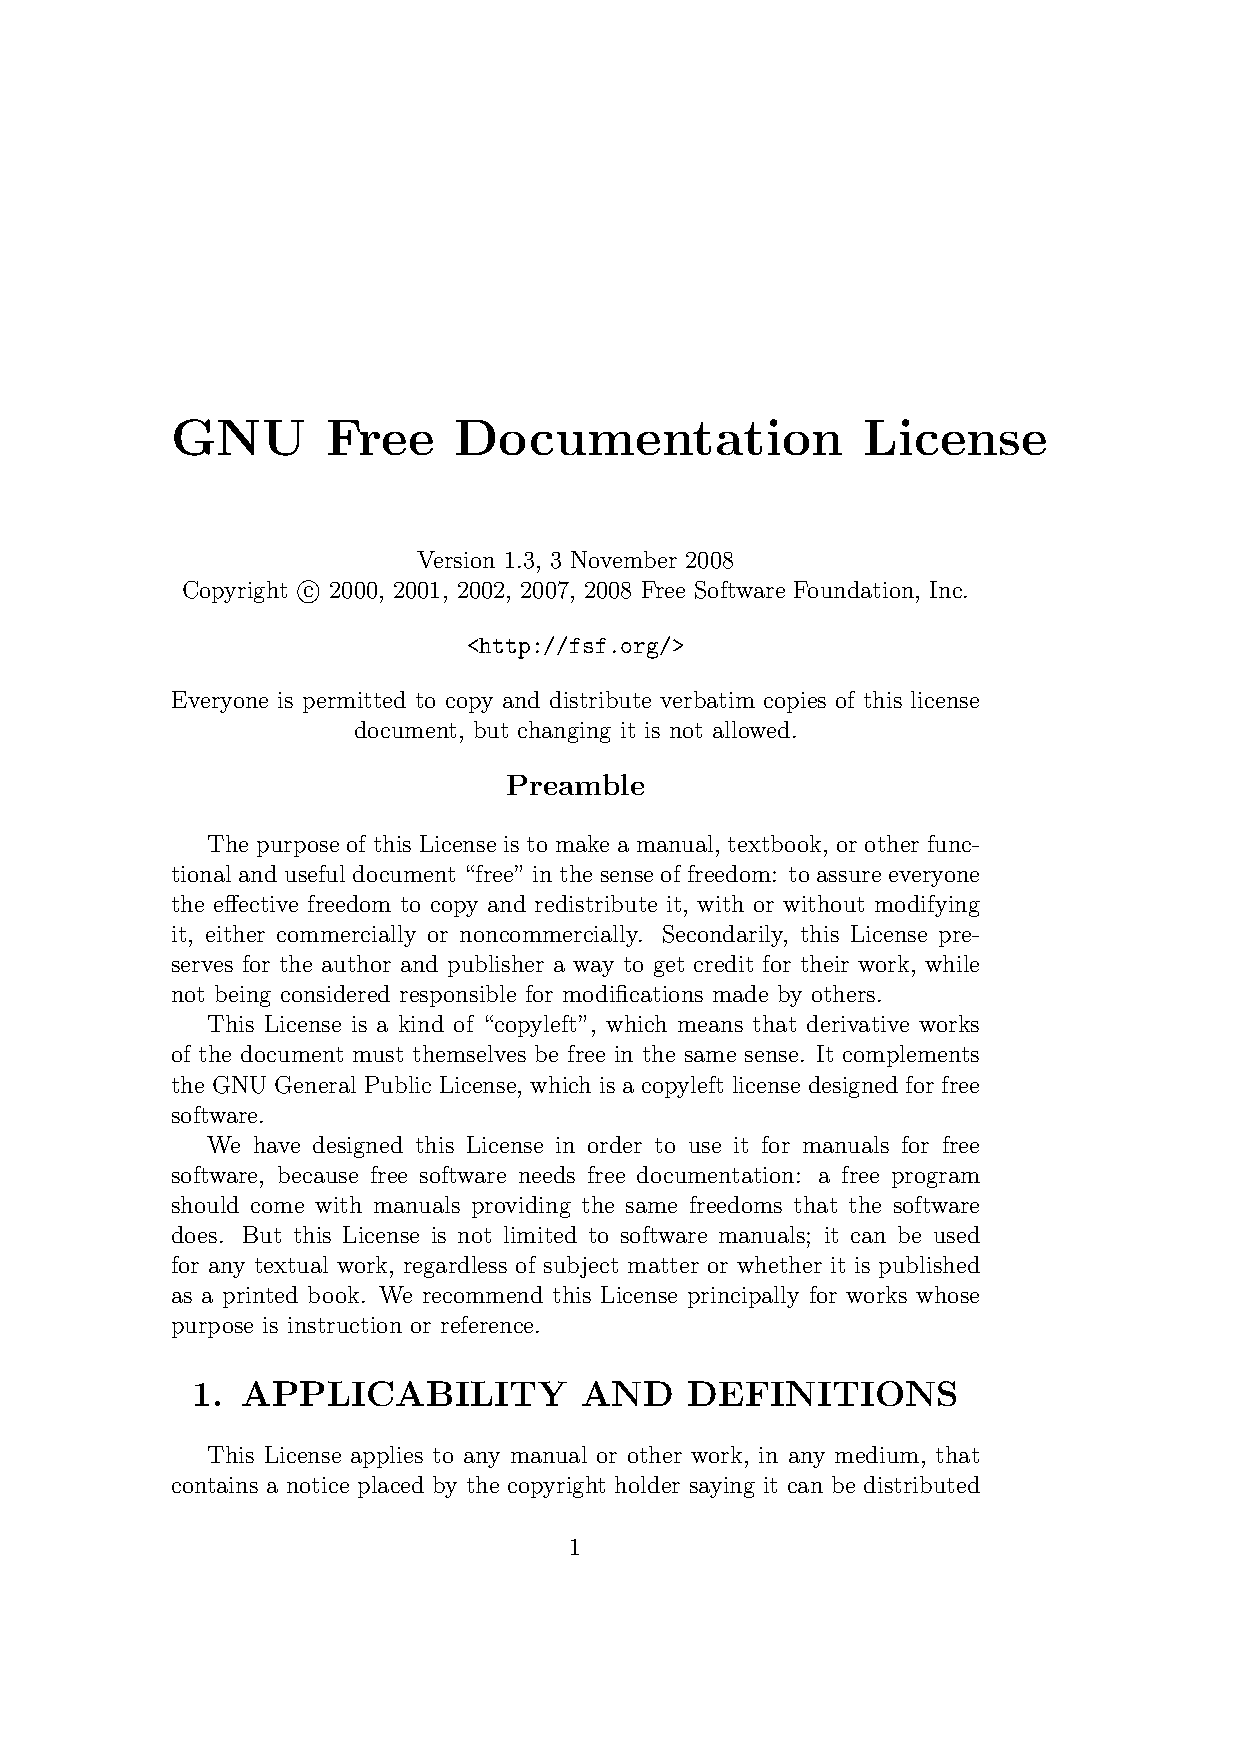
\includepdf[pages=-]{fdl.pdf}

\end{document}
